\documentclass[screen, aspectratio=43]{beamer}
\usepackage[T1]{fontenc}
\usepackage[utf8]{inputenc}

% Use the NTNU-temaet for beamer 
% \usetheme[style=ntnu|simple|vertical|horizontal, 
%     language=bm|nn|en, 
%     smalltitle, 
%     city=all|trondheim|alesund|gjovik]{ntnu2017}
\usetheme[style=ntnu,language=en]{ntnu2017}

\usepackage[english]{babel}
\usepackage[style=numeric,backend=biber,natbib=false,sorting=none]{biblatex}

\title[HCI-intro]{Human Computer Interaction}
\subtitle{Evaluation in HCI}
\author[A. Xamb{\'o}]{Anna Xamb{\'o}}
\institute[NTNU]{Department of Music, NTNU}
\date{25 October 2018}
%\date{} % To have an empty date

\addbibresource{../hci-lectures.bib} % Add bibliography database

% Set the reference style to numeric.
% See here: http://tex.stackexchange.com/questions/68080/beamer-bibliography-icon
\setbeamertemplate{bibliography item}[text] 

% Set bibliography fonts to a small size.
\renewcommand*{\bibfont}{\footnotesize}

\begin{document}

\begin{frame}
  \titlepage
\end{frame}

% Alternatively, special title page command to get a different background
% \ntnutitlepage

\begin{frame}
\frametitle{Learning Outcomes}
\begin{itemize}
\item Understand the trends in the approach to evaluation in the CHI conference / HCI discipline.
\item Establish connections between quantitative, qualitative and mixed research methods from HCI applied to interactive music systems.
\item Conceptualize an approach to evaluation of a self-built musical instrument.
\item Discover the research methods and evaluation elements in a successful CHI paper submission.
\end{itemize}
\end{frame}
%
\begin{frame}
\frametitle{Preparation: Reading}
\begin{itemize}
\item Send a summary (1 page max.) of the following article:
\begin{itemize}
\item From Mice to Men - 24 years of Evaluation in CHI~\cite{Barkhuus.Rode.2007.evalchi}\\
\url{http://barkhu.us/barkhuus-altchi2007.pdf} 
\end{itemize}
The summary should include: the main topic of the paper, the approach used, the main findings, and the main contributions.
\end{itemize}
\end{frame}
%
\begin{frame}
\frametitle{Class Structure}
\begin{itemize}
\item 10.15-10.30 Group discussion about the prep. reading.
\item 10:30-10:45 Presentation/lecture.
\item 10.45-11.05 Group discussion about own research questions.
\item 11.10-11.40 Team group discussion: research methods of the selected CHI best paper.
\item 11.40-12.00 Closing: what makes a good CHI paper? 
\end{itemize}
\end{frame}
%
\begin{frame}
\frametitle{Group discussion: ``From Mice to Men - 24 years of Evaluation in CHI''}
\begin{itemize}
\item Any surprises? 
\item Any limitations? 
\item Is the title accurate?
\end{itemize}
\end{frame}
%
\begin{frame}
\frametitle{Is it familiar...?}
\begin{figure}
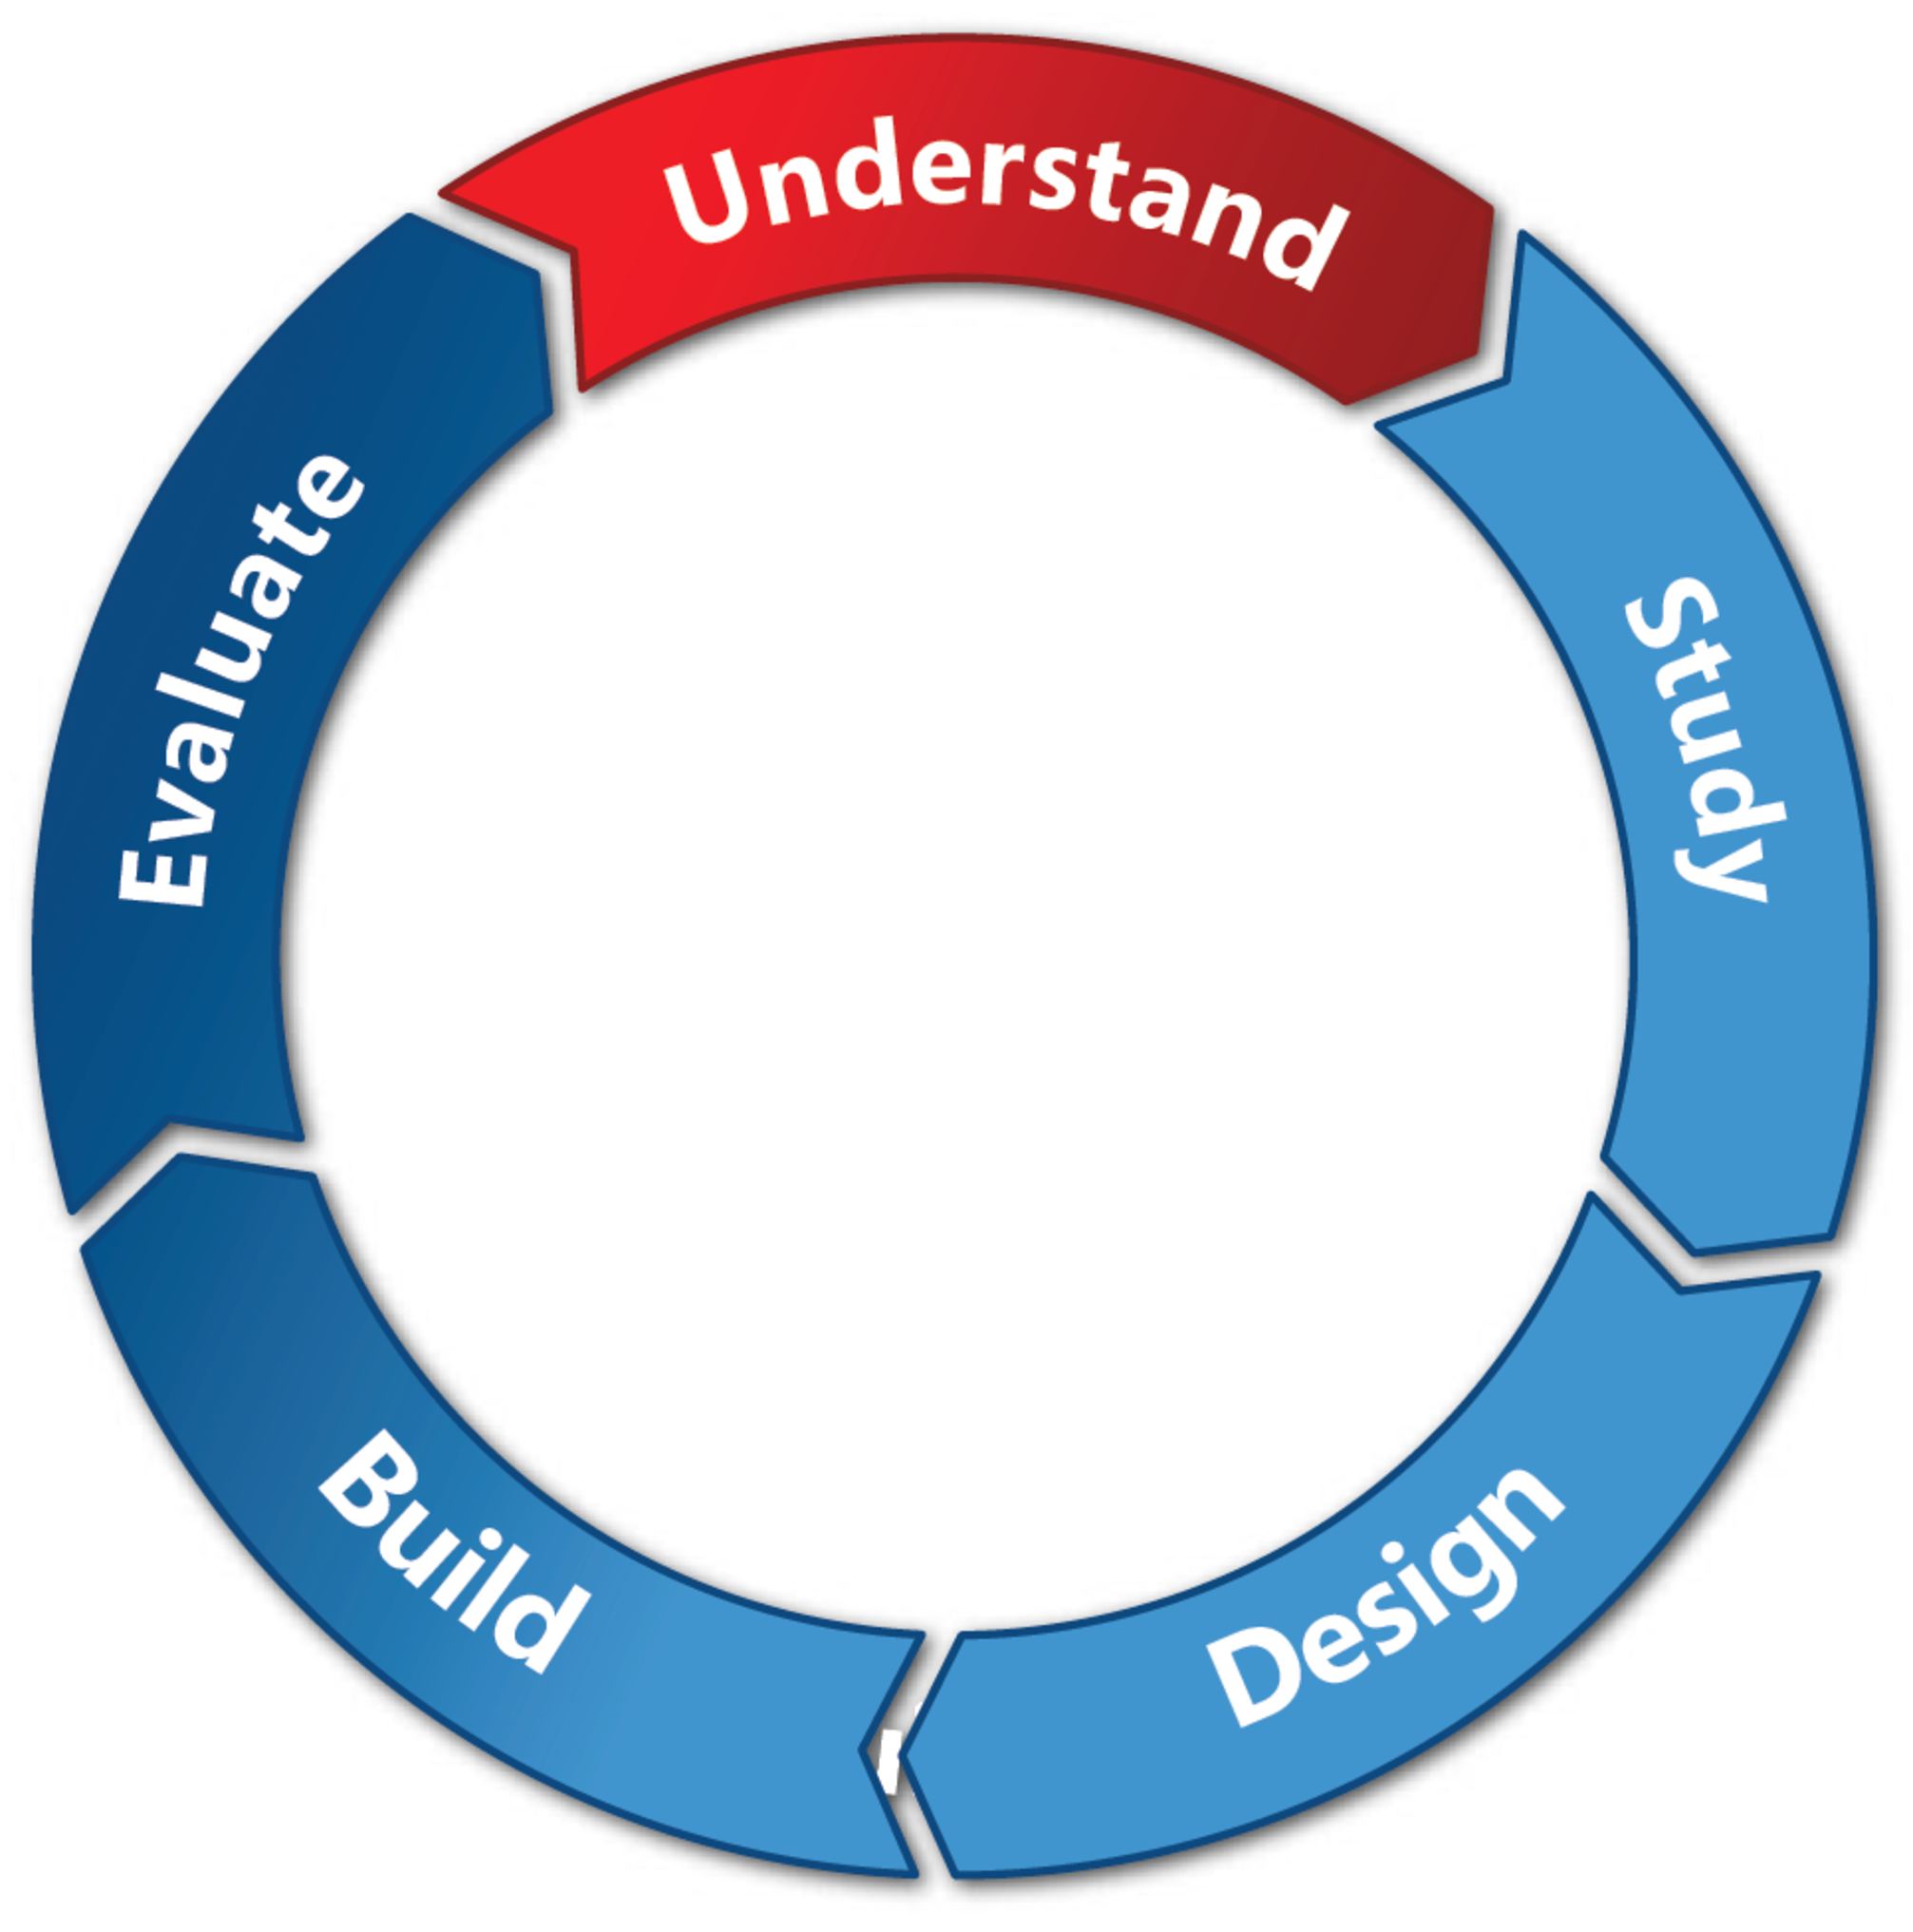
\includegraphics[scale=0.20]{img/design-cycle.pdf}
\end{figure}
\end{frame}
%
\begin{frame}
\frametitle{The research and design cycle}
\begin{figure}
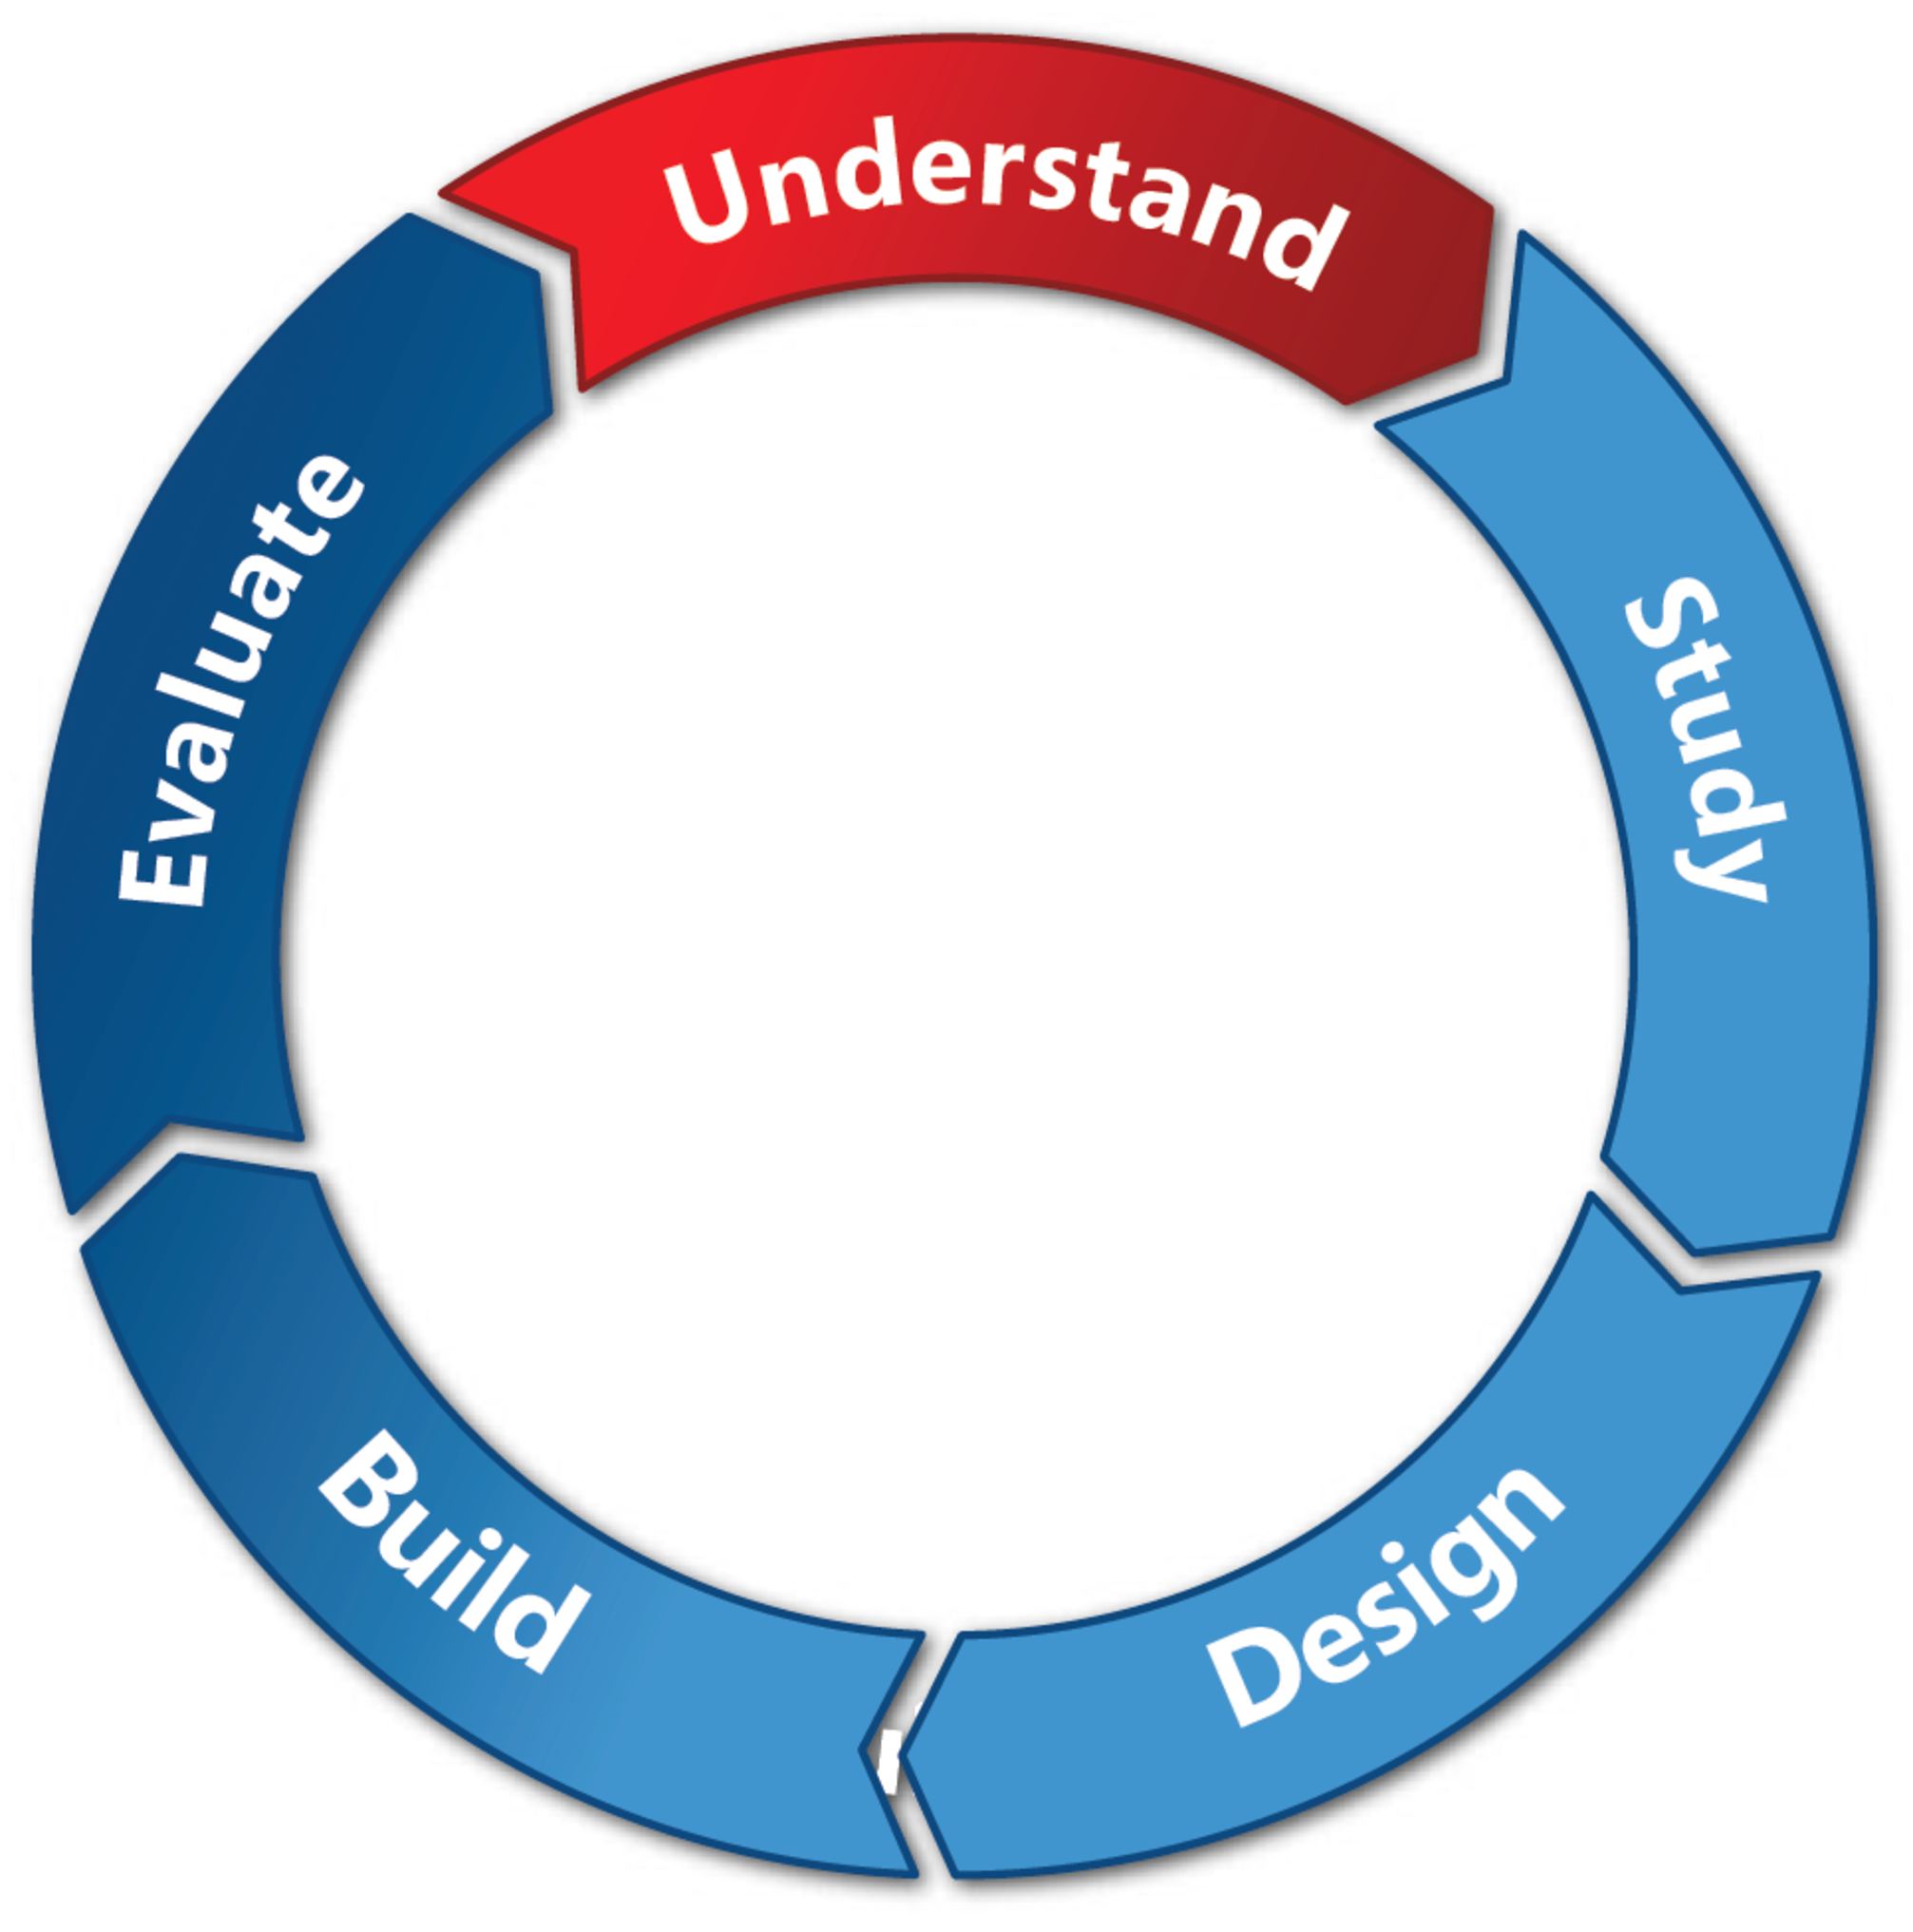
\includegraphics[scale=0.20]{img/design-cycle.pdf}
\caption{Extended user-centred, five-stage design/research model \cite{Harper.et.al.2008.being}}
\end{figure}
\end{frame}
%
\begin{frame}
\frametitle{Presentation/lecture: Design and evaluation of interactive tabletops for music performance}
A case study of an approach to quantitative, qualitative and mixed research methods from HCI applied to interactive music systems: 
\begin{itemize}
\item Tabletop Tangible Interfaces for Music Performance: Design and Evaluation \cite{Xambo.2015.thesis}
\end{itemize}
\end{frame}
%
\begin{frame}
\frametitle{Group discussion: What is your research question?}
Potential ways of evaluating the music hacks considering quantitative, qualitative, and mixed research methods...
\begin{itemize}
\item What are the challenges? 
\item What are the limitations of each approach? 
\item What would be a research questions that fits the three groups? 
\item Who would be your users? 
\end{itemize}
\end{frame}
%
\begin{frame}
\frametitle{Team group discussion: What are the research methods?}
Selection of the same paper than day 1 (or another if you prefer) from the CHI 2018 Best Papers (\url{https://chi2018.acm.org/attending/best-of-chi/}) and discussion about...
\begin{itemize}
\item whether and how the research methods used fit the trends explained in the prep. reading.
\item why (or why not) it is a successful evaluation.
\end{itemize}
\end{frame}
%
\begin{frame}
\frametitle{Closing: What makes a good CHI paper?}
The teams summarize to the group their group discussion about the suitability of the research methods used and what makes a good CHI paper.
\end{frame}
%
\begin{frame}
\frametitle{What makes a good CHI paper?: Mindmap}
\end{frame}
%
%
\begin{frame}
\frametitle{Human-Computer Interaction Day 2 - Group Assignment (post-class)}
\begin{itemize}
\item Send a summary (1 page max.) of the research methods used in the selected article discussed in group during class on Tuesday 23 October 2018, from the CHI 2018 Best Papers (\url{https://chi2018.acm.org/attending/best-of-chi/}) after the class on Thursay 25 October 2018 and before Friday 26 October 2018 9:00. \\
You should explain the research methods used:
\begin{itemize} 
\item are they quantitative, qualitative, or mixed methods? 
\item How are they related with the research question? 
\item What are the limitations of this approach? 
\item How do the authors address the limitations? 
\item What other research methods could have been used instead and why?
\end{itemize}
\end{itemize}
\end{frame}
%
\begin{frame}
\frametitle{Resources}
\begin{itemize}
\item The content of this class can be found on Canvas here:\\
\url{https://uio.instructure.com/courses/11472/pages/human-computer-interaction-1b}
\item The slides of this class can be found on GitHub here: \\
\url{https://github.com/axambo/hci-lecture-slides/tree/master/slides/d2/}
\end{itemize}
\end{frame}
%
\begin{frame}
  \frametitle{References}
  \printbibliography
\end{frame}
%
\end{document}
